\subsection{Gazebo}

The Gazebo is the oldest simulator among Bullet and Mujoco. The development of Gazebo dates back to the 2002 University of Southern California. Later, Willow Garage took over and extended Gazebo to ROS and PR2. Gazebo became the primary simulation engine of the ROS community. Eventually, in 2012 Gazebo became part of OSRF(Open Source Robotics Foundation)\footnote{\url{https://www.openrobotics.org/}}, a spin-off from Willow Garage.

Technically, Gazebo is a simulation platform, which inherits different physics engines, such as Bullet, ODE\footnote{\url{https://www.ode.org/}}, Simbody\footnote{\url{https://simtk.org/}}, and DART\footnote{\url{https://dartsim.github.io/}}. According to the documentation of Gazebo 11.0, it supports ODE engine default, and other engines can be used if developers compile Gazebo from the source. That means the performance of the overall Gazebo simulation highly depends on those individual physics engine’s performances.  Another dependency of Gazebo is ROS(Robotics Operating System)\footnote{\url{https://www.ros.org/}}. ROS infrastructure handles all communication. Thus, users need to rely on ROS to interact with Gazebo. We believe this assumption is too large. Even if relying on ROS can bring many well-structured tools, learning ROS has a steep curve and can cause a large overhead for simple projects.
Nonetheless, developers invested highly on neat and clean documentation to reduce the overhead for new users. We consider the documentation and tutorials as a merit of the open-source project. Correspondingly, being open source contributes hugely to a large community willing to support, answering questions on forums, and submitting pull requests for possible bug fixes. 

According to Pitonakova et al., Gazebo has usability issues due to not having a 3D mesh editing option and difficulties of installing dependencies for third party models. They also noted that Gazebo performs reasonably well in large simulation environments, so it could be more convenient to conduct extensive swarm robotics experiments on Gazebo \cite{Pitonakova2018}.  

Based on our experiments in \ref{fig:GazeboPR2}, we found that Gazebo provides useful models to set up a table-top environment for robotics picking applications quickly. Although we have not performed any grasping experiments on Gazebo, editing the size, position, and orientation of models directly on simulation GUI is a useful feature, lacking both on Pybullet and Mujoco.


\begin{figure}

    \begin{subfigure}{0.49\textwidth}
      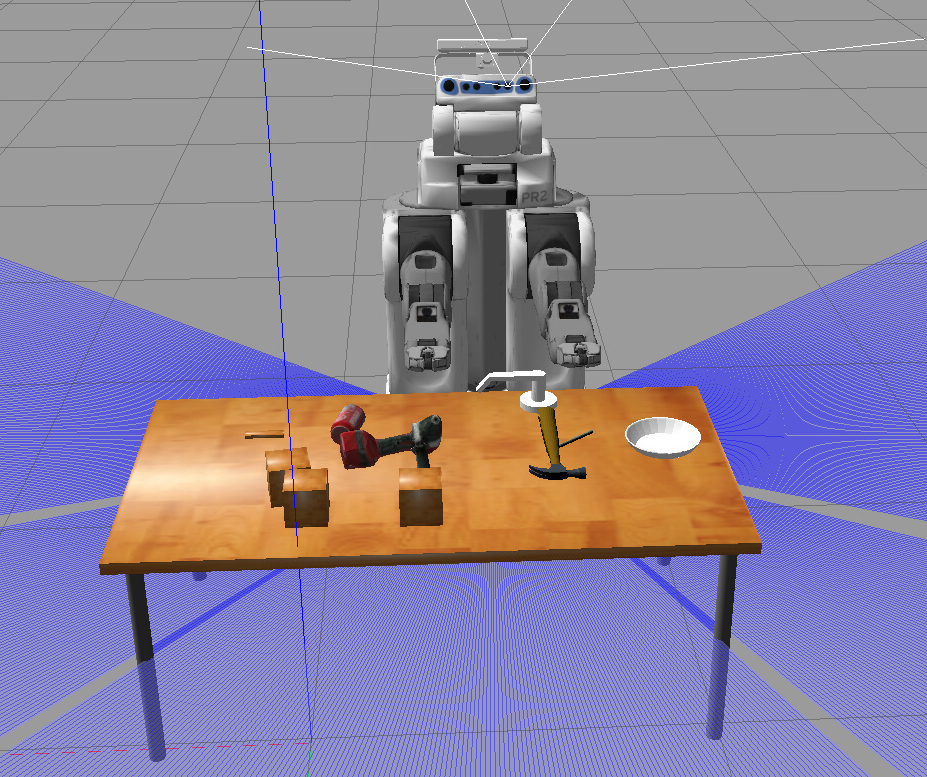
\includegraphics[width=\linewidth]{figures/GazeboEnv1.png}
      \caption{} \label{fig:1a}
    \end{subfigure}%
    \hspace*{\fill}   % maximize separation between the subfigures
    \begin{subfigure}{0.49\textwidth}
      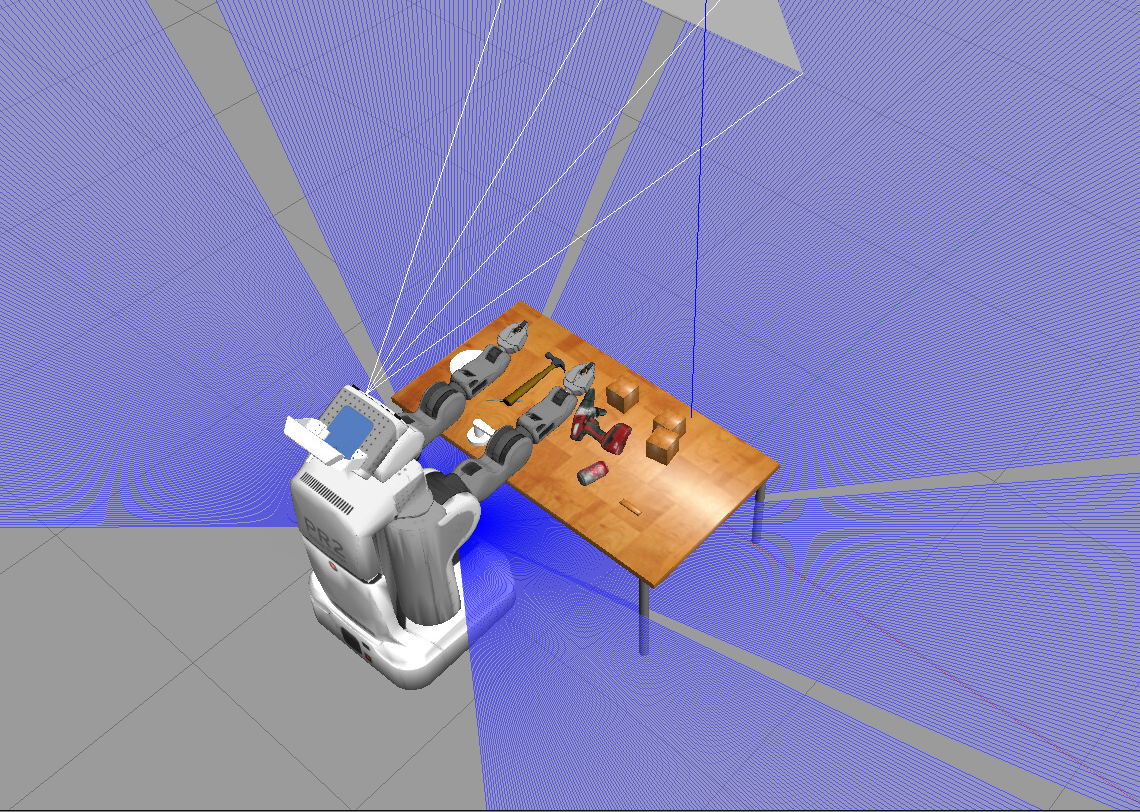
\includegraphics[width=\linewidth]{figures/GazeboEnv2.png}
      \caption{} \label{fig:1b}
    \end{subfigure}%

\caption{Table-top environment in Gazebo simulation with variety of objects and PR2 robot \label{fig:GazeboPR2}}
\end{figure}